% !TEX encoding = UTF-8 Unicode
%!TEX root = thesis.tex
% !TEX spellcheck = en-US
%%=========================================
\addcontentsline{toc}{section}{Introduction}
\section*{Introduction}
For decades, music technology has made music more appealing by applying audio effects, which are processing techniques that alter audio so that it sounds different. For example, one common audio effect in rock music is distortion on the electric guitars, which will make them sound “fuzzy” instead of “clean”. Some audio effects become more appealing when their parameters are changed over time. For example, there is the auto-wah effect, which essentially is a peaking filter, which amplifies a specific frequency and cuts off other frequencies. The volume of the input is used to dynamically control the cutoff frequency of the filter. When the cutoff frequency is swept from low to high, it sounds like “wah”, hence the name auto-wah. The auto-wah effect is an example of an adaptive audio effect (Verfaille \& Arfib, 2006). Since meaningful interactions between musical elements can make music more interesting and appealing, cross-adaptive audio effects were invented. In this class of audio effects, parameters are dynamically informed by features of other sounds. In the 1960s, Stockhausen presented one of the first cross-adaptive audio effects in his composition “Hymnen” (Moritz, 2003), where he, amongst other things, modulated the rhythm of one anthem with the harmony of another anthem. Sidechain compression is a more recent example of a cross-adaptive audio effect. In that technique, the amplitude of one sound controls one or more parameters in the compressor that is applied to a different sound. In electronic music, sidechain compression is often used to let the volume of the bass drum turn down the volume of the bass synth. This is done to avoid conflicts between the bass drum and the bass synth, and also provides a pulsating, rhythmic dynamic to the sound. Further, cross-adaptive audio effects have been used in algorithms for mixing multichannel audio (Reiss, 2011) and voice-controlled synthesizers (Cartwright \& Pardo, 2014). Generally, cross-adaptive audio effects can be applied in a wide range of research fields, including live music performance and audio mastering. Current research at the Music Technology department at Norwegian University of Science and Technology aims at exploring radically new modes of musical interaction in live music performance. In 2015, Øyvind Brandtsegg presented a toolkit for experimenting with signal interaction. This toolkit enables one to find musically interesting signal interactions by empirical experimentation. However, this can be tedious due to the vast number of combinations. Also, while most low-level audio features are mathematically and acoustically well defined, it’s hard to use them for musically interesting cross-adaptive audio effects. One often needs to combine several audio features in complex ways. An audio feature can be linked to any effect parameter, and the mapping function can be anything. A setup can have many instruments, lots of audio effects, and the ordering of the effects may vary. Indeed, Brandtsegg’s suggestions for future work includes “practical and musical exploration of the technique, and the mapping between sound features and effects controls”. As cross-adaptive audio effects are relatively uncharted territory, methods to evaluate various cross-couplings of features have not been formalized. There is a need for a tool that can help efficiently search for useful mappings in those huge search spaces. That was the spark of this project.

\begin{figure}[h]
    \centering
    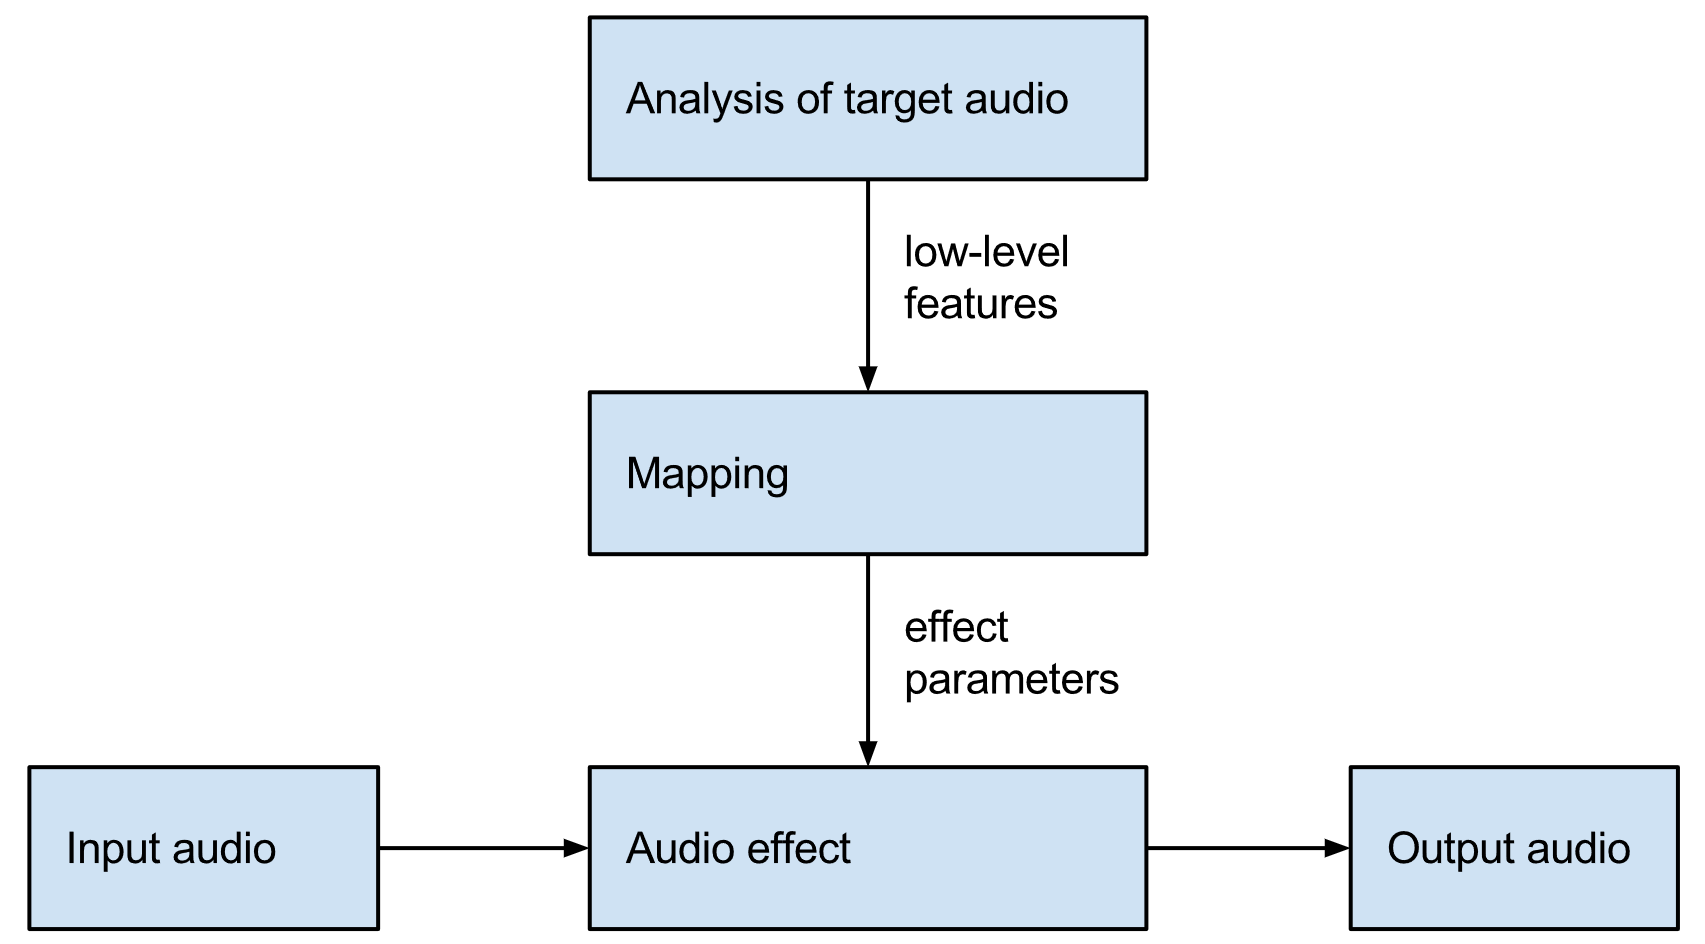
\includegraphics[width=0.6\textwidth]{01_simple_signal}
    \caption{Cross-adaptive audio effect process with two audio streams: input audio and target audio}
    \label{fig:mesh1}
\end{figure}

In practice, a music performance that uses cross-adaptive audio effects can be a very complex, dynamic system with many signal interactions. However, to limit the scope and complexity of the problem, this project will study signal interactions between only two sounds at a time: an input sound and a target sound. A single audio effect is applied to the input sound. The parameters of this effect are dynamically informed by features from the target audio. The goal of the tool implemented in this project is to make interesting mappings from target audio analysis to audio effect parameters. Brandtsegg (2015) suggested that machine learning can be useful in this context. Generally, for a machine learning problem to be well-defined, a performance measure is needed. A good performance measure would be “how appealing does it sound?”. However, what generally sounds appealing to humans is tacit knowledge and cannot be simply described mathematically. Because there are no good objective measures of what a good cross-adaptive audio effect is, an assumption has been made in this project: If a cross-adaptive audio effect makes features of one sound audible in the other sound, then it is considered interesting. Therefore it has been decided that the objective of the system in this project should be to make the input sound similar to the target sound.

The mapping (figure 1.1) is a function that maps n-dimensional vectors (audio features) to m-dimensional vectors (effect parameters). Artificial neural networks are apt for this, as they can approximate a wide variety of continuous functions (Hornik, 1991). Backpropagation (Werbos, 1982; Lecun, Buttou, Orr, \& Müller, 1998) is an efficient algorithm for training neural networks (i.e. finding a set of useful weights for it), but it requires target values for the output nodes to compute error signals. Since no sets of target values are available for this project, and there is generally no good way of telling exactly how the mapping affects the resulting sound, it makes sense to use evolutionary computation to train the neural networks instead. That is feasible because it is possible to construct a fitness function that returns a score based on how similar two sounds are. All in all, this project is about developing a toolkit that explores evolutionary computation in various ways to evolve artificial neural networks that act as mappings in cross-adaptive audio effects.

As the developed system has many components and deals with lots of numbers in the form of audio features, neural network weights, audio effect parameters, output sounds and fitness values, it’s hard to understand what the system really does. To alleviate this, a significant part of the project has been about developing a comprehensive interactive visualization system as a part of the toolkit. One motivation for this is that one cannot improve the optimization process if one does not know where it fails. It was also made in order to make the toolkit more human-understandable and to make evaluation of results more efficient.
